% -*- latex -*-
%%%%%%%%%%%%%%%%%%%%%%%%%%%%%%%%%%%%%%%%%%%%%%%%%%%%%%%%%%%%%%%%
%%%%%%%%%%%%%%%%%%%%%%%%%%%%%%%%%%%%%%%%%%%%%%%%%%%%%%%%%%%%%%%%
%%%%
%%%% This text file is part of the source of
%%%% `Parallel Programming in MPI and OpenMP'
%%%% by Victor Eijkhout, copyright 2012-2022
%%%%
%%%% omp-affinity.tex : thread affinity
%%%%
%%%%%%%%%%%%%%%%%%%%%%%%%%%%%%%%%%%%%%%%%%%%%%%%%%%%%%%%%%%%%%%%
%%%%%%%%%%%%%%%%%%%%%%%%%%%%%%%%%%%%%%%%%%%%%%%%%%%%%%%%%%%%%%%%

\index{thread!affinity|(}

\Level 0 {OpenMP thread affinity control}
\label{sec:omp-proc-bind}

The matter of thread affinity becomes important on \emph{multi-socket nodes}%
\index{affinity!thread!on multi-socket nodes};
see the example in section~\ref{sec:first-touch}.

Thread placement can be controlled with two environment variables:
\begin{itemize}
\item the environment variable \indexompshow{OMP_PROC_BIND}
  describes how threads are bound to \indextermbus{OpenMP}{places}; while
\item the variable \indextermtt{OMP_PLACES} describes these places
  in terms of the available hardware.
\item When you're experimenting with these variables it is a good idea
  to set \indextermtt{OMP_DISPLAY_ENV} to true, so that OpenMP will
  print out at runtime how it has interpreted your specification.
  The examples in the following sections will display this output.
\end{itemize}

\Level 1 {Thread binding}
\label{omp:threadbind}

The variable \indexompdef{OMP_PLACES} defines a series of places to
which the threads are assigned,
and \indexompdef{OMP_PROC_BIND} describes how threads are tied to those places.

Typical values for \indexompshow{OMP_PLACES} are
\begin{itemize}
\item \indexompshow{socket}: threads are bound to a \indexterm{socket}, but can be
  moved between cores in the socket;
\item \indexompshow{core}: threads are bound to a \indexterm{core}, but
  can be moved between hyperthreads in the core;
\item \indexompshow{thread}: threads are bound to a specific \indexterm{hyper-thread}.
\end{itemize}

Values for \indexompshow{OMP_PROC_BIND} are implementation-defined,
but typically:
\begin{itemize}
\item \indexompshow{master}: threads are bound to the same place as the master thread;
\item \indexompshow{close}: subsequent thread numbers are placed close together
  in the defined places;
\item \indexompshow{spread}: subsequent thread numbers are maxially spread over places;
\item \indexompshow{true}: threads are bound to their initial placement;
\item \indexompshow{false}: threads are not bound to their initial placement;
\end{itemize}
where the values \lstinline{master,close,spread} are ordained by the standard,
and the others depend on the implementation.

There is no runtime function for setting the binding, but the \ac{ICV} \indexompshow{bind-var}
can be retrieved with \indexompshow{omp_get_proc_bind}.
The binding can also be set with the \indexompclause{proc_bind} clause
on the \lstinline{parallel} directive,
with values \lstinline{master,close,spread}.

Example: if you have two sockets and you define
\begin{verbatim}
OMP_PLACES=sockets
\end{verbatim}
then
\begin{itemize}
\item thread 0 goes to socket 0,
\item thread 1 goes to socket 1,
\item thread 2 goes to socket 0 again,
\item and so on.
\end{itemize}
On the other hand, if the two sockets have a total of sixteen cores
and you define
\begin{verbatim}
OMP_PLACES=cores
OMP_PROC_BIND=close
\end{verbatim}
then
\begin{itemize}
\item thread 0 goes to core 0, which is on socket~0,
\item thread 1 goes to core 1, which is on socket~0,
\item thread 2 goes to core 2, which is on socket~0,
\item and so on, until thread 7 goes to core 7 on socket~0, and
\item thread 8 goes to core 8, which is on socket~1,
\item et cetera.
\end{itemize}
The value \n{OMP_PROC_BIND=close} means that the assignment goes
successively through the available places.
The variable \n{OMP_PROC_BIND} can also be set to \n{spread}, which
spreads the threads over the places.
With
\begin{verbatim}
OMP_PLACES=cores
OMP_PROC_BIND=spread
\end{verbatim}
you find that
\begin{itemize}
\item thread 0 goes to core 0, which is on socket~0,
\item thread 1 goes to core 8, which is on socket~1,
\item thread 2 goes to core 1, which is on socket~0,
\item thread 3 goes to core 9, which is on socket~1,
\item and so on, until thread 14 goes to core 7 on socket~0, and
\item thread 15 goes to core 15, which is on socket~1.
\end{itemize}

So you see that \n{OMP_PLACES=cores} and \n{OMP_PROC_BIND=spread} very
similar to \n{OMP_PLACES=sockets}. The difference is that the latter
choice does not bind a thread to a specific core, so the operating
system can move threads about, and it can put more than one thread on
the same core, even if there is another core still unused.

The value \n{OMP_PROC_BIND=master} puts the threads in the same place
as the master of the team. This is convenient if you create teams
recursively. In that case you would use the \indexclause{proc\_bind}
clause rather than the environment variable, set to \n{spread} for the
initial team, and to \indexpragma{master} for the recursively created team.

\Level 1 {Effects of thread binding}
\label{sec:omp:bindeffect}

Let's consider two example program. First we consider the program for
computing~$\pi$, which is purely compute-bound.

\begin{tabular}{rrrr}
  \toprule
  \#threads&\n{close/cores}&\n{spread/sockets}&\n{spread/cores}\\
  \midrule
   1& 0.359& 0.354& 0.353\\
   2& 0.177& 0.177& 0.177\\
   4& 0.088& 0.088& 0.088\\
   6& 0.059& 0.059& 0.059\\
   8& 0.044& 0.044& 0.044\\
  12& 0.029& 0.045& 0.029\\
  16& 0.022& 0.050& 0.022\\
  \bottomrule
\end{tabular}

We see pretty much perfect speedup for the \n{OMP_PLACES=cores}
strategy; with \n{OMP_PLACES=sockets} we probably get occasional
collisions where two threads wind up on the same core.

Next we take a program for computing the time evolution of the
\indexterm{heat equation}:
\[ t=0,1,2,\ldots\colon \forall_i\colon
x^{(t+1)}_i = 2x^{(t)}_i-x^{(t)}_{i-1}-x^{(t)}_{i+1}
\]
This is a bandwidth-bound operation because the amount of computation
per data item is low.

\begin{tabular}{rrrr}
  \toprule
  \#threads&\n{close/cores}&\n{spread/sockets}&\n{spread/cores}\\
  \midrule
   1& 2.88& 2.89& 2.88\\
   2& 1.71& 1.41& 1.42\\
   4& 1.11& 0.74& 0.74\\
   6& 1.09& 0.57& 0.57\\
   8& 1.12& 0.57& 0.53\\
  12& 0.72& 0.53& 0.52\\
  16& 0.52& 0.61& 0.53\\
  \bottomrule
\end{tabular}

Again we see that \n{OMP_PLACES=sockets} gives worse performance for
high core counts,
probably because of threads winding up on the same core.
The thing to observe in this example is that with 6~or~8 cores the
\n{OMP_PROC_BIND=spread} strategy gives twice the performance of
\n{OMP_PROC_BIND=close}.

The reason for this is that a single socket
does not have enough bandwidth for all eight cores on the
socket. Therefore, dividing the eight threads over two sockets gives
each thread a higher available bandwidth than putting all threads on
one socket.

\Level 1 {Place definition}

There are three predefined values for the \indexompshow{OMP_PLACES}
variable: \n{sockets, cores, threads}. You have already seen the first
two; the \n{threads} value becomes relevant on processors that have
hardware threads. In that case, \n{OMP_PLACES=cores} does not tie a
thread to a specific hardware thread, leading again to possible
collisions as in the above example. Setting \n{OMP_PLACES=threads}
ties each OpenMP thread to a specific hardware thread.

There is also a very general syntax for defining places that uses a
\begin{verbatim}
  location:number:stride
\end{verbatim}
syntax. Examples:
\begin{itemize}
\item
\begin{verbatim}
OMP_PLACES="{0:8:1},{8:8:1}"
\end{verbatim}
  is equivalent to
  \n{sockets} on a two-socket design with eight cores per socket: it
  defines two places, each having eight consecutive cores. The threads
  are then places alternating between the two places, but not further
  specified inside the place.
\item The setting \n{cores} is equivalent to
\begin{verbatim}
OMP_PLACES="{0},{1},{2},...,{15}"
\end{verbatim}
\item On a four-socket design, the specification
\begin{verbatim}
OMP_PLACES="{0:4:8}:4:1"
\end{verbatim}
  states that the place \n{0,8,16,24} needs to be repeated four times,
  with a stride of one. In other words,  thread~0 winds up on
  core~0 of some socket, the thread~1 winds up on core~1 of some
  socket, et cetera.
\end{itemize}

\Level 1 {Binding possibilities}

Values for \indextermtt{OMP_PROC_BIND} are: \n{false, true, master, close, spread}.
\begin{itemize}
\item false: set no binding \item true: lock threads to a core \item
  master: collocate threads with the master thread \item close: place
  threads close to the master in the places list \item spread: spread
  out threads as much as possible
\end{itemize}

This effect can be made local by
giving the \indexclause{proc\_bind} clause in the
\indexpragma{parallel} directive.

A safe default setting is
\begin{verbatim}
export OMP_PROC_BIND=true
\end{verbatim}
which prevents the operating system from
\indextermsub{migrating a}{thread}. This prevents many scaling problems.

Good examples of \emph{thread placement} on the
\emph{Intel Knight's Landing}%
\index{Intel!Knight's Landing!thread placement}:
\url{https://software.intel.com/en-us/articles/process-and-thread-affinity-for-intel-xeon-phi-processors-x200}

As an example, consider a code where two threads write to a shared
location.
%
\cverbatimsnippet[examples/omp/c/sharing.c]{shareboth}
%
There is now a big difference in runtime depending on how close the
threads are. We test this on a processor with both cores and
hyperthreads. First we bind the OpenMP threads to the cores:
\begin{verbatim}
OMP_NUM_THREADS=2 OMP_PLACES=cores OMP_PROC_BIND=close ./sharing
run time = 4752.231836usec
sum = 80000000.0
\end{verbatim}
Next we force the OpenMP threads to bind to hyperthreads inside one core:
\begin{verbatim}
OMP_PLACES=threads OMP_PROC_BIND=close ./sharing
run time = 941.970110usec
sum = 80000000.0
\end{verbatim}
Of course in this example the inner loop is pretty much meaningless
and parallelism does not speed up anything:
\begin{verbatim}
OMP_NUM_THREADS=1 OMP_PLACES=cores OMP_PROC_BIND=close ./sharing
run time = 806.669950usec
sum = 80000000.0
\end{verbatim}
However, we see that the two-thread result is almost as fast, meaning
that there is very little parallelization overhead.

\index{thread!affinity|)}

\Level 0 {First-touch}
\label{sec:first-touch}

The affinity issue shows up in the \indexterm{first-touch}
phenomemon.

%%packtsnippet firsttouch

A little background knowledge. Memory is organized in
\indextermbus{memory}{page}s\index{page, memory|see{memory, page}},
and what we think of as `addresses' really are
\indextermsub{virtual}{address}es,
mapped to \indextermsub{physical}{address}es
through a \indextermbus{page}{table}.

This means that data in your program can be anywhere in physical memory.
In particular, on a \indextermsub{dual}{socket} node,
the memory can be mapped to either of the sockets.

The next thing to know is that
memory allocated with \indextermtt{malloc} and like
routines is not immediately mapped; that only happens when data is
written to it. In light of this, consider the following OpenMP code:
\begin{lstlisting}
double *x = (double*) malloc(N*sizeof(double));

for (i=0; i<N; i++)
  x[i] = 0;

#pragma omp parallel for
for (i=0; i<N; i++)
  .... something with x[i] ...
\end{lstlisting}
Since the initialization loop is not parallel it is executed by the
main thread, making all the memory associated with the socket of
that thread.
Subsequent access by the other socket will then access
data from memory not attached to that socket,
which induces a considerable delay, and performance degradation.

\Level 1 {Example}

Let's consider an example. We make the initialization
parallel subject to an option:
%
\cverbatimsnippet{heatinitfirst}

If the initialization is not parallel, the array will be mapped
to the socket of the master thread; if it is parallel,
it may be mapped to different sockets, depending on where the threads run.

As a simple application
we run a heat equation, which is parallel,
though not embarassingly so:
%
\cverbatimsnippet{heatmethodrun}

On the \indextermbus{TACC}{Frontera} machine, with dual 28-core
\indextermbus{Intel}{Cascade Lake} processors,
we use the following settings:

\begin{lstlisting}[language=bash]
export OMP_PLACES=cores
export OMP_PROC_BIND=close
# no parallel initialization
make heat && OMP_NUM_THREADS=56 ./heat
# yes parallel initialization
make heat && OMP_NUM_THREADS=56 ./heat 1
\end{lstlisting}

This gives us a remarkable difference in runtime:
\begin{itemize}
\item
  Sequential init: avg=2.089, stddev=0.1083
\item
  Parallel init: avg=1.006, stddev=0.0216
\end{itemize}
This large difference will be mitigated
for algorithms with higher arithmetic intensity.

\begin{exercise}
  How do the OpenMP dynamic schedules relate to this issue?
\end{exercise}

\Level 1 {Solution in C++}

\lstset{language=C++}

The problem with realizing first-touch in \emph{C++}%
\index{C++!first-touch|see{first-touch, in C++}}%
\index{first-touch!in C++}
is that \lstinline+std::vector+ fills its allocation with default values.
This is known as `value-initialization', and it makes
\begin{lstlisting}
vector<double> x(N);
\end{lstlisting}
equivalent to the non-parallel allocation and initialization above.

Here is a solution.
\begin{cppnote}{Uninitialized containers}
  \label{cpp:uninitial}
  Default initialization is a problem.
  We make a template for uninitialized types:
  %
  \cxxverbatimsnippet{cppuninitial}

  so that we can create vectors that behave normally:
  %
  \cxxverbatimsnippet{cppuninitialvec}
\end{cppnote}

Running the code with the regular definition of a vector,
and the above modification,
reproduces the runtimes of the C~variant above.

Another option is to wrap memory allocated with \lstinline{new}
in a \lstinline+unique_ptr+:
%
\cxxverbatimsnippet{newuninitial}

Note that this gives fairly elegant code,
since square bracket indexing is overloaded for \lstinline+unique_ptr+.
The only disadvantage is that we can not query the \lstinline{size}
of these arrays. Or do bound checking with \lstinline{at},
but in high performance contexts that is usually not appropriate anyway.

%%packtsnippet end

\lstset{language=C}

\begin{comment}
\begin{exercise}
  \label{ex:first-touch}
  Finish the following fragment and run it with first all the cores of
  one socket, then all cores of both sockets. (If you know how to do
  explicit placement, you can also try fewer cores.)
\begin{lstlisting}
  for (int i=0; i<nlocal+2; i++)
    in[i] = 1.;
  for (int i=0; i<nlocal; i++)
    out[i] = 0.;

  for (int step=0; step<nsteps; step++) {
#pragma omp parallel for schedule(static)
    for (int i=0; i<nlocal; i++) {
      out[i] = ( in[i]+in[i+1]+in[i+2] )/3.;
    }
#pragma omp parallel for schedule(static)
    for (int i=0; i<nlocal; i++)
      in[i+1] = out[i];
    in[0] = 0; in[nlocal+1] = 1;
  }
\end{lstlisting}
\end{exercise}
\end{comment}

\Level 1 {Remarks}

You could move pages with \indextermtt{move_pages}.

By regarding affinity,
in effect you are adopting an \ac{SPMD} style of programming.
You could make this explicit by having each thread allocate its part
of the arrays separately, and storing a private pointer as
\indexpragma{threadprivate}~\cite{Liu:2003:OMP-SPMD}. However, this
makes it impossible for threads to access each other's parts of the
distributed array, so this is only suitable for
total \indextermsub{data}{parallel} or
\indextermsub{embarrassingly}{parallel} applications.

\begin{comment}
[c202-002 c:1] export OMP_PLACES=cores
[c202-002 c:2] export OMP_PROC_BIND=close
[c202-002 c:3] make heat && OMP_NUM_THREADS=56 ./heat
make: `heat' is up to date.
Time=  2.0048 #ops=2.000e+09 on 56 threads
[c202-002 c:4] make heat && OMP_NUM_THREADS=56 ./heat
make: `heat' is up to date.
Time=  2.2479 #ops=2.000e+09 on 56 threads
[c202-002 c:5] make heat && OMP_NUM_THREADS=56 ./heat
make: `heat' is up to date.
Time=  1.9717 #ops=2.000e+09 on 56 threads
[c202-002 c:6] make heat && OMP_NUM_THREADS=56 ./heat
make: `heat' is up to date.
Time=  2.1107 #ops=2.000e+09 on 56 threads
[c202-002 c:7] make heat && OMP_NUM_THREADS=56 ./heat
make: `heat' is up to date.
Time=  2.1087 #ops=2.000e+09 on 56 threads
[c202-002 c:8] make heat && OMP_NUM_THREADS=56 ./heat 1
make: `heat' is up to date.
Parallel init
Time=  1.0420 #ops=2.000e+09 on 56 threads
[c202-002 c:9] make heat && OMP_NUM_THREADS=56 ./heat 1
make: `heat' is up to date.
Parallel init
Time=  0.9962 #ops=2.000e+09 on 56 threads
[c202-002 c:10] make heat && OMP_NUM_THREADS=56 ./heat 1
make: `heat' is up to date.
Parallel init
Time=  1.0077 #ops=2.000e+09 on 56 threads
[c202-002 c:11] make heat && OMP_NUM_THREADS=56 ./heat 1
make: `heat' is up to date.
Parallel init
Time=  0.9939 #ops=2.000e+09 on 56 threads
[c202-002 c:12] make heat && OMP_NUM_THREADS=56 ./heat 1
make: `heat' is up to date.
Parallel init
Time=  0.9880 #ops=2.000e+09 on 56 threads
\end{comment}

\Level 0 {Affinity control outside OpenMP}

There are various utilities to control process and thread placement.

Process placement can be controlled on the Operating system level by
\indextermttdef{numactl}
\begin{tacc}
(the TACC utility \indextermttdef{tacc_affinity} is a wrapper around this)
\end{tacc}
on Linux (also \indextermtt{taskset}); Windows
\indextermtt{start/affinity}.

Corresponding system calls: \indextermtt{pbing} on Solaris,
\indextermtt{sched_setaffinity} on Linux,
\indextermtt{SetThreadAffinityMask} on Windows.

Corresponding environment variables: \indextermtt{SUNW_MP_PROCBIND} on
Solaris, \indextermtt{KMP_AFFINITY} on Intel.

The \emph{Intel compiler}\index{Intel!compiler!thread affinity} has an
environment variable for affinity control:
\begin{verbatim}
export KMP_AFFINITY=verbose,scatter
\end{verbatim}
values: \n{none,scatter,compact}

For \emph{gcc}\index{gcc!thread affinity}:
\begin{verbatim}
export GOMP_CPU_AFFINITY=0,8,1,9
\end{verbatim}

For the \indextermbus{Sun}{compiler}:
\begin{verbatim}
SUNW_MP_PROCBIND
\end{verbatim}

\Level 0 {Tests}
\label{sec:loop-affinity}

We take a simple loop and consider the influence of binding parameters.

\cverbatimsnippet{ompsineloop}

\Level 1 {Lonestar 6}

Lonestar 6, dual socket \indextermbus{AMD}{Milan}, total 112 cores:
figure~\ref{fig:ls6-bind}.

\begin{figure}[t]
  \tikzsetnextfilename{speedup-ls6}
  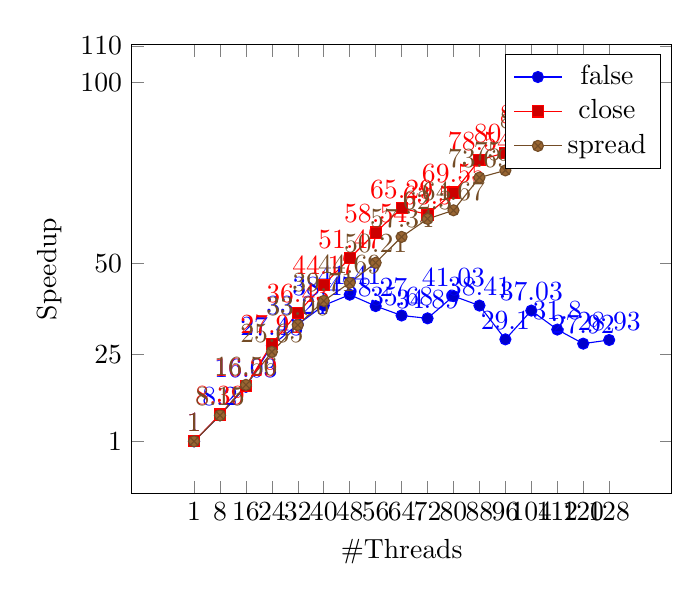
\begin{tikzpicture}  
    \begin{axis}
      [  
        enlargelimits=0.15,
        xlabel={\#Threads},
        ylabel={Speedup},
        symbolic x coords={1,8,16,24,32,40,48,56,64,72,80,88,96,104,112,120,128},
        xtick=data,  ytick={1,25,50,100,110},
        nodes near coords,  
        nodes near coords align={vertical},  
      ]  
      \addplot coordinates {(1, 1.00) (8, 8.20) (16, 16.03) (24, 27.43) (32, 33.21) (40, 38.47) (48, 41.41) (56, 38.27) (64, 35.68) (72, 34.89) (80, 41.03) (88, 38.41) (96, 29.10) (104, 37.03) (112, 31.80) (120, 27.92) (128, 28.93) };
      \addplot coordinates {(1, 1.00) (8, 8.39) (16, 16.29) (24, 27.91) (32, 36.43) (40, 44.17) (48, 51.47) (56, 58.54) (64, 65.29) (72, 63.50) (80, 69.55) (88, 78.54) (96, 80.53) (104, 85.82) (112, 90.17) (120, 93.41) (128, 88.75) };        
      \addplot coordinates {(1, 1.00) (8, 8.15) (16, 16.56) (24, 25.65) (32, 33.06) (40, 39.71) (48, 44.69) (56, 50.21) (64, 57.34) (72, 62.30) (80, 64.67) (88, 73.69) (96, 75.67) (104, 84.61) (112, 88.58) (120, 91.90) (128, 96.04  ) }; 
      \legend{false, close, spread}
    \end{axis}
  \end{tikzpicture}  
  \caption{Speedup as function of thread count, Lonestar 6 cluster, different binding parameters}
  \label{fig:ls6-bind}
\end{figure}

\Level 1 {Frontera}

\indextermbus{Intel}{Cascade Lake}, dual socket, 56 cores total;
figure~\ref{fig:frontera-bind}.

For all core counts to half the total,
performance for all binding strategies seems equal.
After that , \n{close} and \n{spread} perform equally,
but the speedup for the \n{false} value gives erratic numbers.

\begin{figure}[t]
  \tikzsetnextfilename{speedup-frontera}
  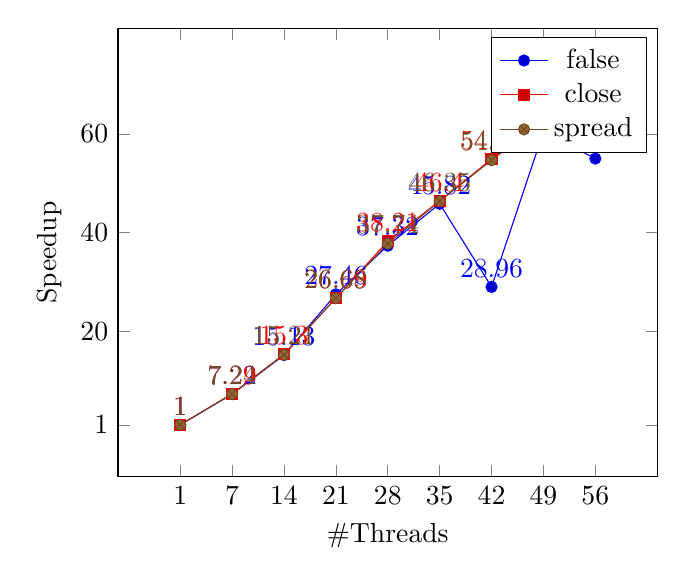
\begin{tikzpicture}  
    \begin{axis}
      [  
        enlargelimits=0.15,
        xlabel={\#Threads},
        ylabel={Speedup},
        symbolic x coords={1,7,14,21,28,35,42,49,56},
        xtick=data,  ytick={1,20,40,60},
        nodes near coords,  
        nodes near coords align={vertical},  
      ]  
      \addplot coordinates {(1, 1.00) (7, 7.22) (14, 15.13) (21, 27.46) (28, 37.32) (35, 45.82) (42, 28.96) (49, 60.41) (56, 54.99) };
      \addplot coordinates {(1, 1.00) (7, 7.29) (14, 15.30) (21, 26.69) (28, 38.21) (35, 46.40) (42, 54.88) (49, 63.04) (56, 70.93) };
      \addplot coordinates {(1, 1.00) (7, 7.24) (14, 15.21) (21, 26.68) (28, 37.74) (35, 46.35) (42, 54.66) (49, 62.61) (56, 70.75) };
      \legend{false, close, spread}
    \end{axis}
  \end{tikzpicture}  
  \caption{Speedup as function of thread count, Frontera cluster, different binding parameters}
  \label{fig:frontera-bind}
\end{figure}

\Level 1 {Stampede2 skylake}

Dual 24-core \indextermbus{Intel}{Skylake};
figure~\ref{fig:skx-bind}.

We see that \n{close} binding gives worse performance than \n{spread}.
Setting binding to \n{false} only gives bad performance for large core counts.

\begin{figure}[t]
  \tikzsetnextfilename{speedup-s2}
  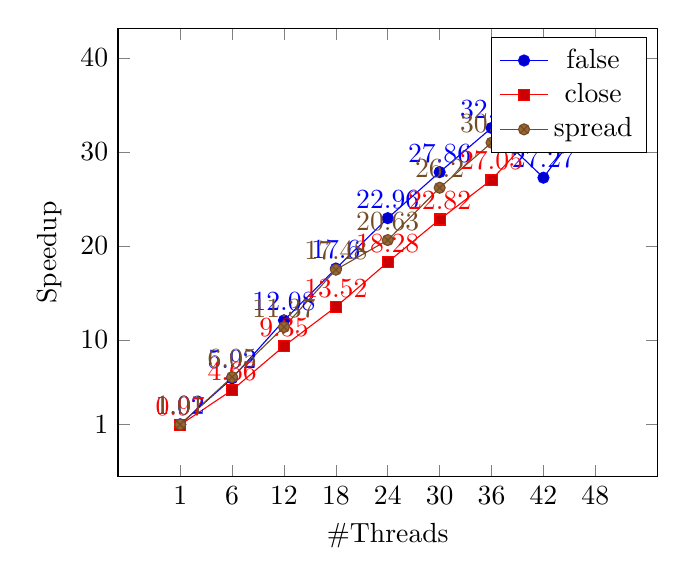
\begin{tikzpicture}  
    \begin{axis}
      [  
        enlargelimits=0.15,
        xlabel={\#Threads},
        ylabel={Speedup},
        symbolic x coords={1,6,12,18,24,30,36,42,48},
        xtick=data,  ytick={1,10,20,30,40,50},
        nodes near coords,  
        nodes near coords align={vertical},  
      ]  
      \addplot coordinates { (1, 1.02) (6, 5.92) (12, 12.08) (18, 17.60) (24, 22.96) (30, 27.86) (36, 32.56) (42, 27.27) (48, 34.78) };
      \addplot coordinates { (1, 0.97) (6, 4.66) (12, 9.35) (18, 13.52) (24, 18.28) (30, 22.82) (36, 27.05) (42, 32.99) (48, 35.13) };
      \addplot coordinates { (1, 1.01) (6, 6.05) (12, 11.37) (18, 17.48) (24, 20.63) (30, 26.20) (36, 30.99) (42, 33.11) (48, 37.67) };
      \legend{false, close, spread}
    \end{axis}
  \end{tikzpicture}  
  \caption{Speedup as function of thread count, Stampede2 skylake cluster, different binding parameters}
  \label{fig:skx-bind}
\end{figure}

\Level 1 {Stampede2 Knights Landing}

We test on a single socket 68-core processor:
the \indextermbus{Intel}{Knights Landing}.

Since this is a single socket design,
we don't distinguish between the \n{close} and \n{spread} binding.
However, the binding value of \n{true} shows good speedup
--~in fact beyond the core count~--
while \n{false} gives worse performance than in other architectures.

\begin{figure}[t]
  \tikzsetnextfilename{speedup-knl}
  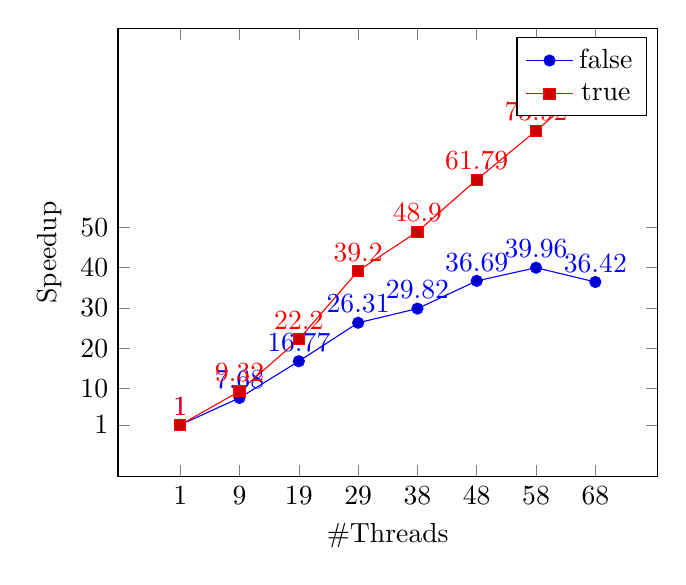
\begin{tikzpicture}  
    \begin{axis}
      [  
        enlargelimits=0.15,
        xlabel={\#Threads},
        ylabel={Speedup},
        symbolic x coords={1,9,19,29,38,48,58,68},
        xtick=data,  ytick={1,10,20,30,40,50},
        nodes near coords,  
        nodes near coords align={vertical},  
      ]  
      \addplot coordinates { (1, 1.00) (9, 7.68) (19, 16.77) (29, 26.31) (38, 29.82) (48, 36.69) (58, 39.96) (68, 36.42) };
      \addplot coordinates { (1, 1.00) (9, 9.32) (19, 22.20) (29, 39.20) (38, 48.90) (48, 61.79) (58, 73.92) (68, 86.52) };
      \legend{false, true}
    \end{axis}
  \end{tikzpicture}  
  \caption{Speedup as function of thread count, Stampede2 Knights Landing cluster, different binding parameters}
  \label{fig:knl-bind}
\end{figure}

\Level 1 {Longhorn}

Dual 20-core \indextermbus{IBM}{Power9}, 4~hyperthreads;
\ref{fig:longhorn-bind}

Unlike the Intel processors, here we use the hyperthreads.
Figure~\ref{fig:longhorn-bind} shows dip in the speedup
at 40 threads.
For higher thread counts the speedup increases to well beyond the
physical core count of~$40$.

\begin{figure}[t]
  \tikzsetnextfilename{speedup-longhorn}
  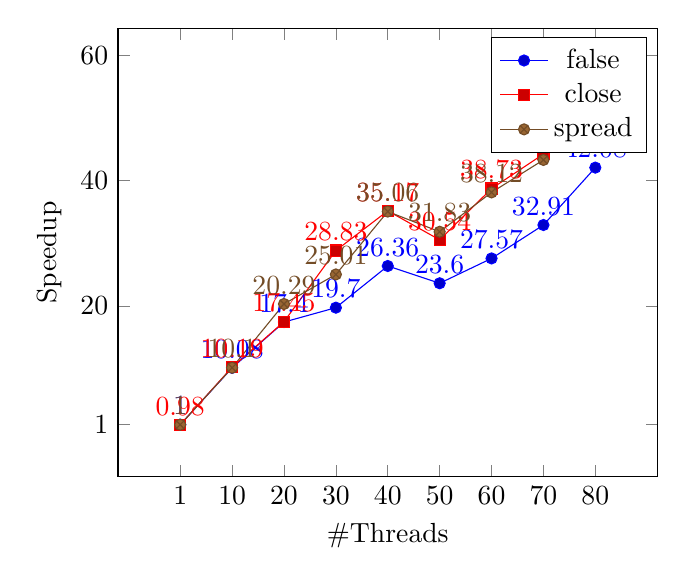
\begin{tikzpicture}  
    \begin{axis}
      [  
        enlargelimits=0.15,
        xlabel={\#Threads},
        ylabel={Speedup},
        symbolic x coords={1,10,20,30,40,50,60,70,80},
        xtick=data,  ytick={1,20,40,60},
        nodes near coords,  
        nodes near coords align={vertical},  
      ]  
      \addplot coordinates { (1, 1.00) (10, 10.08) (20, 17.40) (30, 19.70) (40, 26.36) (50, 23.60) (60, 27.57) (70, 32.91) (80, 42.08) };
      \addplot coordinates { (1, 0.98) (10, 10.19) (20, 17.45) (30, 28.83) (40, 35.17) (50, 30.54) (60, 38.73) (70, 44.24) (80, 56.09) };
      \addplot coordinates { (1, 1.00) (10, 10.10) (20, 20.29) (30, 25.01) (40, 35.06) (50, 31.83) (60, 38.12) (70, 43.31) (80, 56.00) };
      \legend{false, close, spread}
    \end{axis}
  \end{tikzpicture}  
  \caption{Speedup as function of thread count, Longhorn cluster, different binding parameters}
  \label{fig:longhorn-bind}
\end{figure}

